\documentclass[prx,aps,twocolumn,preprintnumbers,amsmath,amssymb,superscriptaddress,showpacs]{revtex4-2}
%\documentclass[aps,prx,twocolumn,showpacs,amsmath,amssymb,superscriptaddress]{revtex4-2}
\usepackage{textcase}
\usepackage{graphicx}
\usepackage{epstopdf}
\usepackage{amsmath}
\usepackage{multirow}
\usepackage{xcolor}
\usepackage{ulem}
%\usepackage[version=4]{mhchem}
\usepackage{float}
\usepackage{array}
\usepackage{booktabs}
%\usepackage{subcaption}

% 命令定义（确保在导言区）
\newcommand{\RNum}[1]{\MakeUppercase{\romannumeral #1}}
\newcommand{\red}{\textcolor {red}}
\newcommand{\green}{\textcolor {green}}
\newcommand{\blue}{\textcolor {blue}}

\begin{document}
%\linenumbers

\title {Supplementary: Identifying the structure of La$_3$Ni$_2$O$_7$ in the pressurized superconducting state}
\author{Hengyuan Zhang}
\thanks{These authors contribute equally to this work.} 
\author{Jielong Zhang}
\thanks{These authors contribute equally to this work.} 
\author{Mengwu Huo}
\author{Junfeng Chen}
\author{Deyuan Hu}
\author{Dao-Xin Yao}
\affiliation{Guangdong Provincial Key Laboratory of Magnetoelectric Physics and Devices, School of Physics, Sun Yat-Sen University, Guangzhou, Guangdong 510275, China}
\author{Hualei Sun}
\affiliation{School of Science, Sun Yat-Sen University, Shenzhen, Guangdong 518107, China}
\author{Kun Cao}
\email{Corresponding author: caok7@mail.sysu.edu.cn}
\affiliation{Guangdong Provincial Key Laboratory of Magnetoelectric Physics and Devices, School of Physics, Sun Yat-Sen University, Guangzhou, Guangdong 510275, China}
\author{Meng Wang}
\email{Corresponding author: wangmeng5@mail.sysu.edu.cn}
\affiliation{Guangdong Provincial Key Laboratory of Magnetoelectric Physics and Devices, School of Physics, Sun Yat-Sen University, Guangzhou, Guangdong 510275, China}


\maketitle

\subsection*{Section 1. Details of the experiments}

\begingroup
\renewcommand{\centering}{\raggedright}
{\subsection{\textbf{\textit{ La$_3$Ni$_2$O$_7$ single crystals growth}} }}
\endgroup

Single crystals of La$_3$Ni$_2$O$_7$  were grown using a high-pressure optical floating zone furnace (model HKZ, SciDre GmbH). The precursor polycrystalline were synthesized by solid-state method. The starting materials of  La$_2$O$_3$ were dried at 1000 °C for 12 hours before use. Stoichiometric amounts of La$_2$O$_3$ and NiO were mixed and sintered at 1200°C for 1 day. Subsequently, the powders were pressed into rods with 6 mm in diameter and 100 mm in length under a hydrostatic pressure and then heated at 1200 °C for 48 hours. Single crystals  La$_3$Ni$_2$O$_7$ were grown by the floating zone method at a rate of 4 mm/h in flowing O$_2$ atmosphere at a pressure of 20 bar and 15 bar, respectively.

\begingroup
\renewcommand{\centering}{\raggedright}
{\subsection{\textbf{\textit{High-pressure electric transport measurements}} }}
\endgroup

We performed electrical transport measurements on La$_3$Ni$_2$O$_7$ crystals under high pressure by using a miniature diamond anvil cell (DAC) constructed from a Be-Cu alloy. The DAC utilized diamond anvils with culets about 300 $\mu$m and an insulating gasket chamber, 100 $\mu$$m$ in diameter, composed of a cubic boron nitride and epoxy mixture. The four-probe van der Pauw technique was applied for the electrical measurements, which were executed with the KBr as a pressure-transmitting medium (PTM).  The high-pressure resistance of a La$_3$Ni$_2$O$_7$ single crystal from 8.8 GPa to 18.9 GPa, as shown in Fig. S1.
\renewcommand{\thefigure}{S\arabic{figure}}
\setcounter{figure}{0}
\begin{figure}[h]
  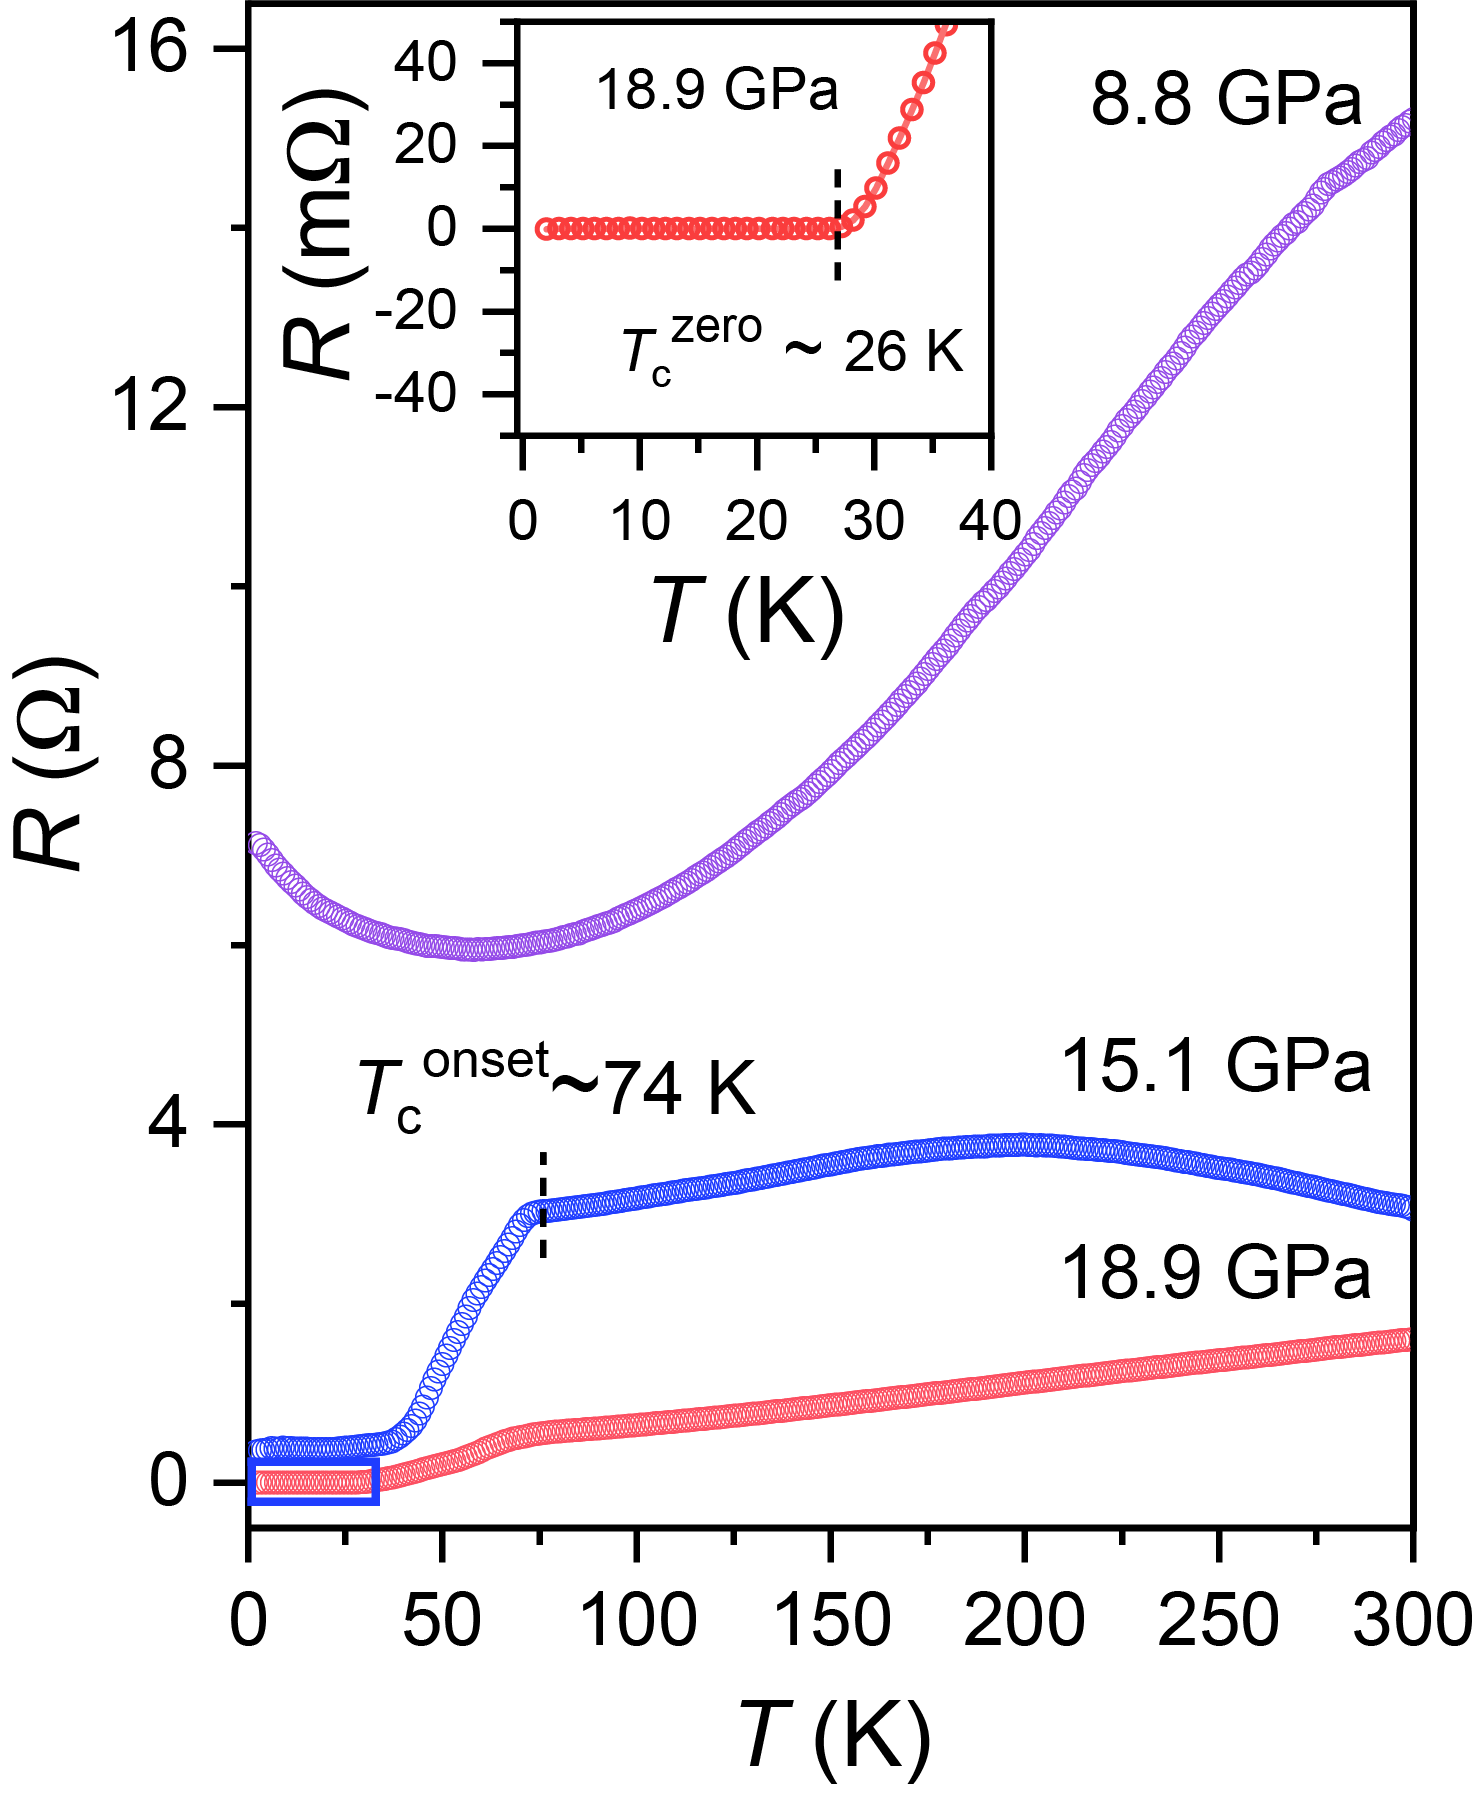
\includegraphics[width=0.4\textwidth]{figures/FigureS1.png}
  \caption{ The high-pressure resistance curves of La$_3$Ni$_2$O$_7$ single crystals from 8.8 GPa to 18.9 GPa. $T_c^{onset}$ and $T_c^{zero}$ are respectively defined as the onset SC transition temperature and zero resistance temperature. $T_c^{onset}$ =74 K is observed at 15.1 GPa. The inset clearly shows the $T_c^{zero}$ $\sim $ 26 K at 18.9 GPa, which means that high-quality La$_3$Ni$_2$O$_7$ superconducting single crystals have been synthesized.}
     \label{Figure:S1}
\end{figure}

\begingroup
\renewcommand{\centering}{\raggedright}
{\subsection{\textbf{\textit{High-pressure Raman experiments}} }}
\endgroup

Prior to the Raman measurements, we performed a Laue diffraction experiment on the sample to verify that the incident Raman light was perpendicular to the $ab$-plane, as illustrated in Fig. S2.


\begin{figure}[h]
  \centering
  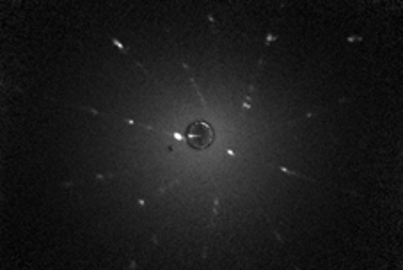
\includegraphics[width=0.4\textwidth]{figures/FigureS2.png}
  \caption{Laue X-ray diffraction for La$_3$Ni$_2$O$_7$. }
   \label{Figure:S2}
\end{figure}

High pressure was generated using a symmetric diamond anvil cell (DAC) with 300 $\mu$m culet. A rhenium gasket with the central 200 $\mu$m hole drilled by laser milling was used as the sample chamber. Hyperbaric Ne gas or He gas was fed into the sample chamber as the pressure transmission medium to keep hydrostatic pressure environment. After pressurization and sealing, the hole diameter shrank to approximately 100 $\mu$m. 

 The Raman spectrum was acquired using a confocal geometry (MoniVist a CRS3) equipped with the Princeton Instrument HRS-500 spectrometer and 633 nm laser as the excitation source. A grating with 1200 g/mm was used to achieve high energy resolution for the phonon lines, providing an energy resolution of 1.5 cm$^{-1}$. The laser power was controlled below 3 mW to minimize the heating effect. A $\times$ 20 objective lens (Zeiss, 0.25 NA) was used to focus the laser beam onto the sample and to collect the scattered light (back scattering geometry). The spectrometer was equipped with a nitrogen-cooled CCD detector. The DAC was placed on the thermal conduction stage of an Optical Magnetic Cryostat (Quantum Design) to enable temperature control from 2-300 K. Resistive temperature sensor (Cernox, Quantum Design) was attached near the sample chamber to measure temperature. The thermometer covers a range from 0.1 K to 420 K, meeting the experiment's required measurement precision. The optical observation window of the Optical Magnetic Cryostat can be coupled to the Raman apparatus to perform low-temperature Raman measurements. Temperature-dependent Raman spectra of  La$_3$Ni$_2$O$_7$ at 5 GPa and 17 GPa are provided in Fig. S3. Notably, no polarizer or analyzer was inserted into the optical path. Therefore, the unpolarized Raman spectrum includes information from all polarization channels. The $L+G$ (Lorentzian with Gaussian) function was used to describe the phonon lines. For the temperature-dependent spectra, the Bose-Einstein factor is divided for comparison.

In all high-pressure experiments, the pressure was jointly monitored by ruby fluorescence (0-15 GPa) and high-frequency edge of the diamond phonon (above 10 GPa). 

\begin{figure}[h]
  \centering
  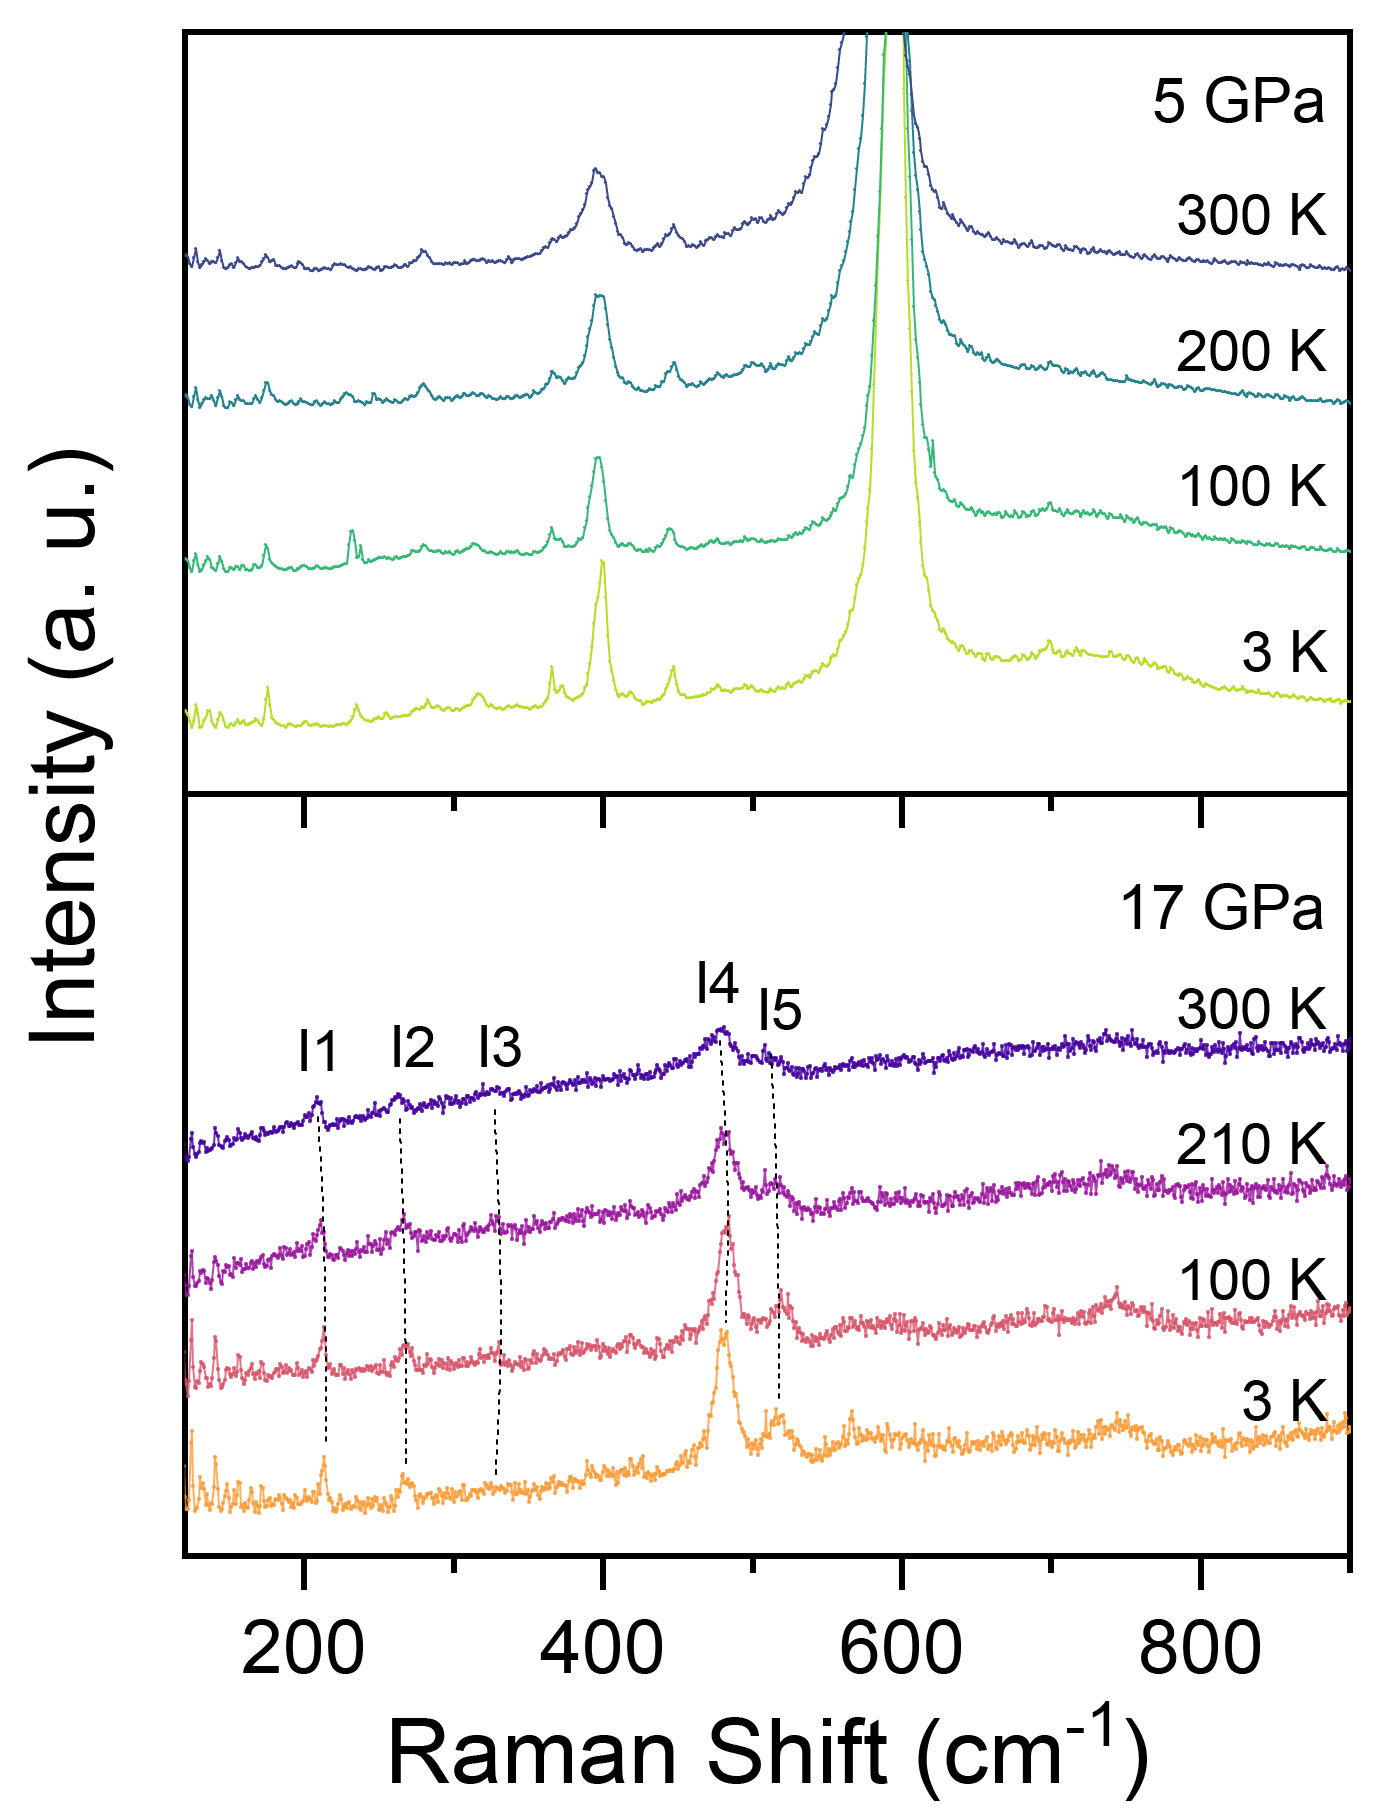
\includegraphics[width=0.4\textwidth]{figures/FigureS3.png}
  \caption{Temperature-dependent Raman spectra of La$_3$Ni$_2$O$_7$ at 5 GPa and 17 GPa.}
     \label{Figure:S3}
\end{figure}

\begingroup
\renewcommand{\centering}{\raggedright}
\subsection*{Section 2. The effective detection depth for Raman and Synchrotron XRD}
\begingroup
\renewcommand{\centering}{\raggedright}
{\subsection{\textbf{\textit{The effective detection depth for Raman}} }}
\endgroup
Since the theoretical expressions for the effective probing depth of Raman scattering are already reported in the literature\cite{Borowicz2016}, we only present here the primary formulas and the derivation of the effective depth specifically for La$_3$Ni$_2$O$_7$.

The absorption of material is described by Lambert law:
\begin{equation}
I(l) = I_0 e^{-\alpha l}
\label{eq:einstein}
\end{equation}
where $I_{0}$ denotes the intensity of incident light, $l$ is the optical  pathway through the material, $I(l)$ is the intensity of the light after the pathway equal to $l$, and $\alpha$ is the absorption coefficient of the material. $\alpha$ can be expressed as a function of imaginary parts of complex refractive index $k$ (or be called damping coefficient) by following equation: 
\begin{equation}
 \alpha = \frac{4\pi k}{\lambda}
\label{eq:einstein}
\end{equation}
where $k$ denote imaginary parts of complex refractive index, is functions of wavelength $\lambda$. Penetration depth $\delta$ is defined as thickness of absorbing material which corresponds to the decrease of the quantity describing electromagnetic wave by $e$ times——  in Eq.(1), $\alpha l=1$. So, the $\delta$ can be described as :
\begin{equation}
\delta = \frac{\lambda}{4\pi k} = \alpha^{-1}
\label{eq:einstein}
\end{equation}
Integrate the intensity of scattered light $I(l)$over the material thickness $l$ to obtain the total scattering intensity.:
\begin{equation}
I(l) = I_0 \varphi_0 \int_{0}^{l} e^{-2\alpha z} \, dz = I_0 \varphi_0 \frac{1 - e^{-2\alpha l}}{2\alpha}.
\label{eq:einstein}
\end{equation}
In Eq. (4) $I_{0}$ denotes the intensity of excitation and $\varphi_{0}$ describes the efficiency of the observed Raman effect. Integration from 0 to $l$ gives the intensity of Raman scattering measured from the layer whose thickness is equal to $l$. The expression $e^{-2\alpha z}$ under the integral described the statistical weight of the contribution of the scattering coming from the material placed at the depth equal to $z$. Factor 2 in the argument of exponential function in Eq. (4) was introduced because scattered light is absorbed in the same manner as exciting light. If $l\to \infty$, we can get $I_{max} =  I_0 \varphi_0 \frac{1 }{2\alpha}$. For a fixed material ( $k$  known), once the $\lambda$ is set, the material’s $\delta$  is fixed. For now, assume that the effective probing depth $\delta_{\text{eff}}^{\text{max}}$ = $n \delta$, we can estimate the value of $n$:  

\begin{equation}
\frac{I(n \delta)}{I_{max}}= \frac{I_0 \varphi_0 \frac{1 - e^{-2\alpha (n \delta)}}{2\alpha}}{I_0 \varphi_0 \frac{1 }{2\alpha}}=1 - e^{-2\alpha (n \delta)}=1 - e^{-2n }.
\label{eq:einstein}
\end{equation} 

when $n=3 ,\frac{I(3 \delta)}{I_{max}}\approx0.9975$. Further increasing depth results in a signal gain that is smaller than the statistical error of a typical CCD detector (approximately 0.004). So, when we know the  $\delta$, we can estimate the $\delta_{\text{eff}}^{\text{max}}$ = $3 \delta$. Therefore, assuming the absorption coefficient $k$ is known, we determine the material's effective detection depth $\delta_{\text{eff}}^{\text{max}}$. Since the  $k$  for La$_3$Ni$_2$O$_7$ is unknown, while the  $k$  for LaNiO$_3$ has been reported ($k$ = 0.69 )\cite{2001Ultraviolet}. The LaNiO$_3$ and La$_3$Ni$_2$O$_7$ share the same chemical elements and have similar chemical densities. Therefore we use the $k$  of  LaNiO$_3$ to replace that of La$_3$Ni$_2$O$_7$. In our experiment, $\lambda$ = $ 633\ nm$.  According to the Eq.(3), we can get the  $\delta( La_3Ni_2O_7)=73\ nm$, and $\delta_{\text{eff}}^{\text{max}}(  La_3Ni_2O_7) =219\ nm$. In actual experiments, the effective detection depth of $\delta_{\text{eff}}(  La_3Ni_2O_7)$ may be less more than 219 nm.

\begingroup
\renewcommand{\centering}{\raggedright}
{\subsection{\textbf{\textit{The effective detection depth for Synchrotron XRD}} }}
\endgroup
For synchrotron XRD, the attenuation of light intensity with depth still follows the Lambert-Beer law. However, for high-energy X-rays, the interaction with matter is dominated by the photoelectric effect. Therefore, the absorption capability of matter for X-rays should be described using the linear attenuation coefficient rather than the imaginary part of the complex refractive index:
\begin{equation}
I(l) = I_0 e^{-\mu l}
\label{eq:einstein}
\end{equation}
$\mu$ is linear attenuation coefficient of material. The $\delta$ is defined as the depth at which the X-ray intensity has decayed to $1/e$ of the surface intensity; the formula for this is:
\begin{equation}
\delta = \frac{1}{\mu}
\label{eq:einstein}
\end{equation}
The linear absorption coefficient $\mu$ is determined by the material’s mass absorption coefficient $\mu_m$ and its density $\rho$: 
\begin{equation}
\mu = \rho \times \mu_m
\label{eq:einstein}
\end{equation}
Consider a simple semi-infinite bulk sample. An X-ray beam strikes the sample at an incident angle $\theta_i$. At a certain depth $z$ within the sample, Bragg diffraction occurs on a crystal plane (with a diffraction angle of $\theta_d$). The diffracted X-ray then exits the surface of the sample at the same angle $\theta_d$. We can calculated the incident path $l_i$: $\frac{z}{sin\theta_i}$, emergent path  $l_d$:  $\frac{z}{sin\theta_d}$. The total diffraction intensity is the sum (integral) of contributions from all depths $z$: 
\begin{equation}
\begin{split}
I_{diff} &= \int_0^l dI_{diff} = C I_0 \int_0^l e^{-\mu z(\frac{1}{\sin \theta_i} + \frac{1}{\sin \theta_d})} dz \\
&= C I_0 \frac{1 - e^{-\mu l (\frac{1}{\sin \theta_i} + \frac{1}{\sin \theta_d})} }{\mu  (\frac{1}{\sin \theta_i} + \frac{1}{\sin \theta_d})}
\end{split}
\label{eq:einstein}
\end{equation}
$C$ represents the inherent diffraction capability of this material. If $l\to \infty$, the Eq.(9) is: 
\begin{equation}
I_{max\cdot diff} = \frac{C I_0}{\mu (\frac{1}{\sin \theta_i} + \frac{1}{\sin \theta_d})}
\label{eq:einstein}
\end{equation}
We can still make an approximation similar to that in Eq(5): 
\begin{equation}
\begin{split}
\frac{I(n \delta)_{diff}}{I_{max\cdot diff}}&= \frac{C I_0 \frac{1 - e^{-\mu (n \delta) (\frac{1}{\sin \theta_i} + \frac{1}{\sin \theta_d})} }{\mu  (\frac{1}{\sin \theta_i} + \frac{1}{\sin \theta_d})}}{C I_0\frac{1}{\mu (\frac{1}{\sin \theta_i} + \frac{1}{\sin \theta_i})}}\\
&={1 - e^{-\mu (n \delta) (\frac{1}{\sin \theta_i} + \frac{1}{\sin \theta_d})} }\\
&={1 - e^{-2n  } }
\end{split}
\label{eq:einstein}
\end{equation} 
We assume symmetric diffraction in Eq. (11), and $\theta_i = \theta_d =90^\circ$. The result of  Eq. (11) is  same as that of  Eq. (5), so n = 3. For now, we can derive the maximum detection depth of La$_3$Ni$_2$O$_7$ in synchrotron XRD. For the mass absorption coefficient of composites $\mu_m$, we can compute a weighted average using each component’s mass fraction $w_i$ and its own mass absorption coefficient $\mu_{m,i}$:
\begin{equation}
\mu_m = \sum_i w_i \times \mu_{m,i}
\label{eq:einstein}
\end{equation}
Given wavelength $\lambda=0.6199\ $$\mathring{A}$  (The wavelength come from the BL15U1  beamline of the Shanghai Synchrotron Radiation Facility (SSRF)), the corresponding photon energy $E \approx 20.00 \text{ keV}$. The molar mass of $M(La_3Ni_2O_7)$ is $646.11 { g/mol}$. At 20 keV, the mass attenuation coefficients $\mu_m$ for each element \cite{xcom_nist} are:  $\mu_{m,La}=36.44\ { cm^{2}/g} $, $\mu_{m,Ni}=16.56\ { cm^{2}/g} $, $\mu_{m,O}=0.738\ { cm^{2}/g} $. The mass absorption coefficient  $\mu_m$ of La$_3$Ni$_2$O$_7$ is calculated as: 
\begin{equation}
\begin{split}
\mu_m &= w_{\text{La}} \times \mu_{m,\text{La}} + w_{\text{Ni}} \times \mu_{m,\text{Ni}} + w_{\text{O}} \times \mu_{m,\text{O}} \\
&= 0.6450 \times 36.44 + 0.1817 \times 16.56 + 0.1733 \times 0.738 \\
&\approx 26.64 \text{ cm}^2/\text{g}
\end{split}
\label{eq:einstein}
\end{equation}
La$_3$Ni$_2$O$_7$ has a density of approximately $\rho= 7.1\ {g/ cm^{3}}$, and thelinear absorption coefficient $\mu$  is calculated as:
\begin{equation}
\mu = \rho \times \mu_m = 7.1 \times 26.64 \approx 189.14 \text{ cm}^{-1}
\label{eq:einstein}
\end{equation}

So, the $\delta $ is $\mu ^{-1}$:
\begin{equation}
\delta = \frac{1}{\mu} = \frac{1}{189.14} \approx 0.00529 \text{ cm} = 52.9  \ \mu\text{m}
\label{eq:einstein}
\end{equation}
\begin{equation}
\delta_{max\cdot diff} = 3\times\delta= 158.6  \ \mu\text{m}
\label{eq:einstein}
\end{equation}
It is evident that Raman has an effective detection depth that differs from synchrotron XRD by roughly three orders of magnitude. In high-pressure experiments, where sample thickness is usually less than 50 $\mu$m. So, synchrotron radiation probes the bulk phase, whereas Raman spectroscopy tends to be more sensitive to surface information.
\\
\subsection*{Section 3. Details of the calculations}
{\subsection{\textbf{\textit{Detailed calculation parameters}} }}
\endgroup

\begin{figure}[h]
  \centering
\vspace{1em}
\hspace*{-0.85cm}
  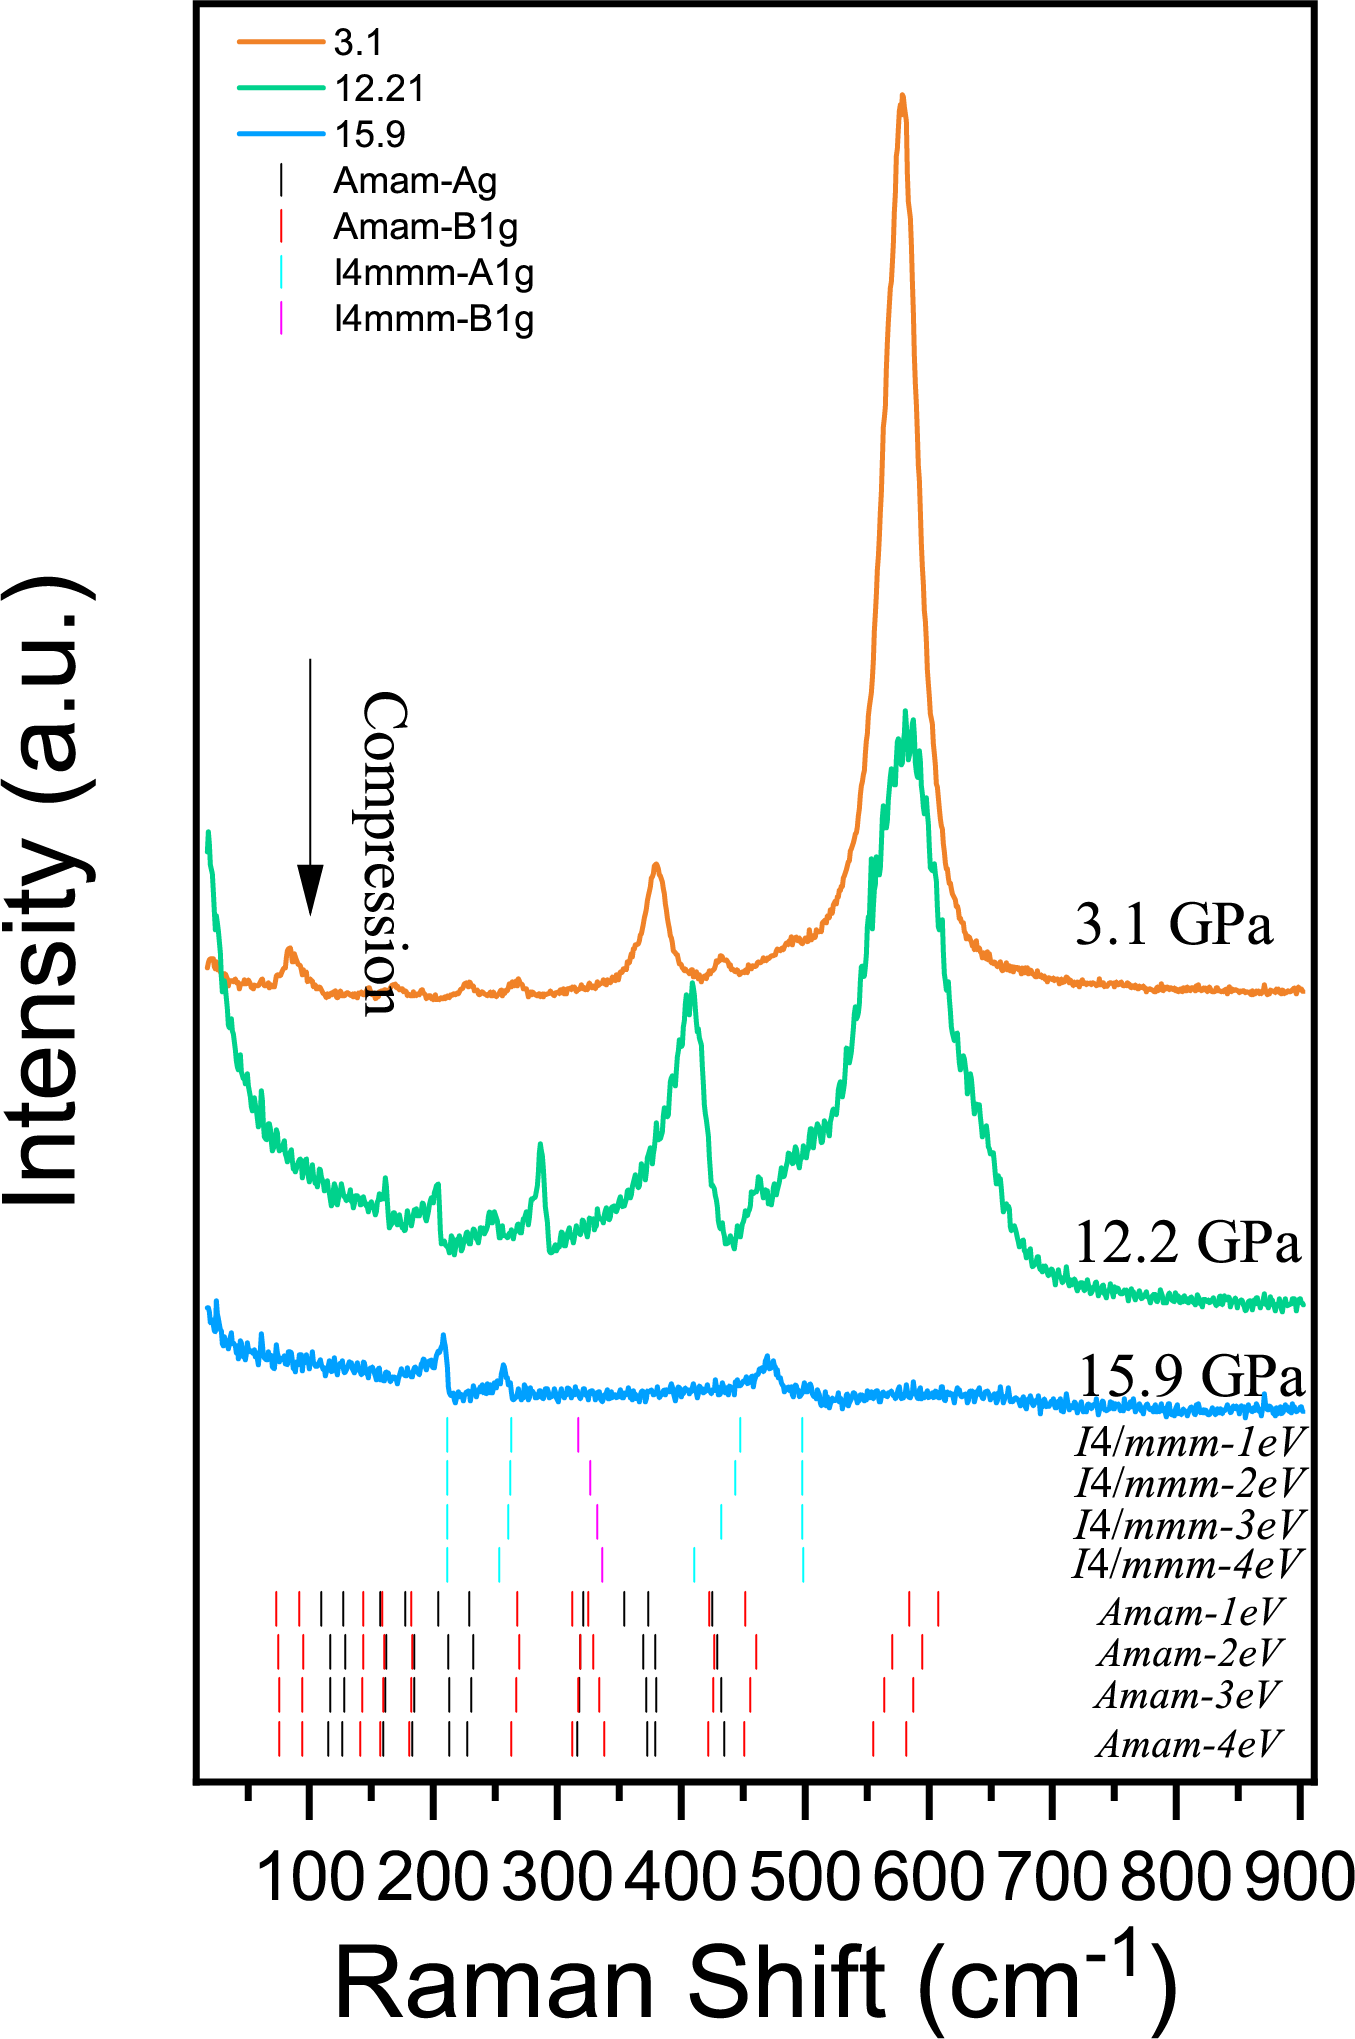
\includegraphics[width=1\columnwidth]{figures/FigureS4.png}
  \caption{Calculated frequencies of Raman active modes with different Hubbard $U$. }
   \label{Figure:S4}
\end{figure}

The projector augmented-wave (PAW) method\cite{PAW} with a kinetic energy cutoff of 500 eV was employed. A $6 \times 6 \times 6$  and a $9 \times 9 \times 9$ (for $Fmmm$ and $I4/mmm$) Monkhorst-Pack $k$-point mesh were used for the $Amam$ and for the $Fmmm$ and $I4/mmm$ phase, respectively. The effective Hubbard $U$ parameter was set to 1 eV (Fig. \ref{Figure:S4}). Atomic positions were relaxed until the atomic forces converged less than 10$^{-2}$ eV/\AA. 

%The effective Hubbard $U=1,2,3,4$ eV were tested considering the general $U$ used for element Ni (Fig. \ref{Figure:S4}). For the $Amam$ phase, the influence of $U$ is primarily concentrated on the highest-frequency phonons, i.e., the major peak A8 or A7. However, for the $I4/mmm$ phase, great shifts in frequency occur. Considering the consistency with the experimental data, especially for the high symmetry $I4/mmm$ phase, we chose $U=1$ eV for DFT calculations.

\begingroup
\renewcommand{\centering}{\raggedright}
{\subsection{\textbf{\textit{Raman tensors}} }}
\endgroup

The Raman tensors are given as\cite{Bilbao}:
\begin{equation}
\nonumber
R_{Amam}: 
\begin{pmatrix}
a & 0 & 0 \\
0 & b & 0 \\
0 & 0 & c
\end{pmatrix}_{A_g},
\begin{pmatrix}
0 & d & 0 \\
d & 0 & 0 \\
0 & 0 & 0
\end{pmatrix}_{B_{1g}},
\end{equation}
\begin{equation}
\nonumber
\begin{pmatrix}
0 & 0 & e \\
0 & 0 & 0 \\
e & 0 & 0
\end{pmatrix}_{B_{2g}},
\begin{pmatrix}
0 & 0 & 0 \\
0 & 0 & f \\
0 & f & 0
\end{pmatrix}_{B_{3g}},
\end{equation}
\begin{equation}
\nonumber
R_{Fmmm}:
\begin{pmatrix}
a & 0 & 0 \\
0 & b & 0 \\
0 & 0 & c
\end{pmatrix}_{A_g},
\begin{pmatrix}
0 & d & 0 \\
d & 0 & 0 \\
0 & 0 & 0
\end{pmatrix}_{B_{1g}},
\end{equation}
\begin{equation}
\nonumber
\begin{pmatrix}
0 & 0 & e \\
0 & 0 & 0 \\
e & 0 & 0
\end{pmatrix}_{B_{2g}},
\begin{pmatrix}
0 & 0 & 0 \\
0 & 0 & f \\
0 & f & 0
\end{pmatrix}_{B_{3g}},
\end{equation}
 \begin{equation}
\nonumber
R_{I4/mmm}:
\begin{pmatrix}
a & 0 & 0 \\
0 & a & 0 \\
0 & 0 & b
\end{pmatrix}_{A_{1g}},
\begin{pmatrix}
c & 0 & 0 \\
0 & -c & 0 \\
0 & 0 & 0
\end{pmatrix}_{B_{1g}},
\end{equation}
\begin{equation}
\nonumber
\begin{pmatrix}
0 & d & 0 \\
d & 0 & 0 \\
0 & 0 & 0
\end{pmatrix}_{B_{2g}},
\begin{pmatrix}
0 & 0 & 0 \\
0 & 0 & e \\
0 & e & 0
\end{pmatrix}_{E_{g}},
\begin{pmatrix}
0 & 0 & e \\
0 & 0 & 0 \\
-e & 0 & 0
\end{pmatrix}_{E_{g}},
\end{equation}


where, in general, the parameters $a,\ b,\ c,\ d,\ e$ and $f$ are distinct for each phase.
\\
\begingroup
\renewcommand{\centering}{\raggedright}
{\subsection{\textbf{\textit{Additional figures}} }}
\endgroup


\begin{figure*}[ht]
    \centering
    \includegraphics[width=1\textwidth]{figures/FigureS5.png}
    \caption{The corresponding modes found in $Fmmm$ and $I4/mmm$ phases to the major peaks (A7 and A8) in $Amam$ phase with close frequencies and similar vibrational patterns. With ir-reps $B_{3g}$ and $E_{g}$ the modes are Raman inactive under our experimental setup.}
    \label{Figure:S5}
\end{figure*}
%\subsection*{Section 3. Additional Figures}
\begin{figure*}[ht]
 \centering
  \includegraphics[width=1\textwidth]{figures/FigureS6.png}
  \caption{Visualization of additional phonon modes. The La atoms with notable vibrations are not omitted. Some vectors are rescaled for display. }
   \label{Figure:S6}
\end{figure*}


\bibliography{reference}

\end{document}
